\documentclass[border=4pt]{standalone}\usepackage[utf8]{inputenc}\usepackage[T1]{fontenc}\usepackage{mathptmx}
\usepackage{tikz}
\usetikzlibrary{arrows.meta,positioning,calc,fit,backgrounds}
\tikzset{>={Stealth[length=2.2mm]}, font=\small,
 blk/.style={draw, line width=0.8pt, fill=white, align=center, inner sep=3pt, text width=#1, minimum height=1.1cm},
 blk/.default=3.0cm,
 iut/.style={fill=black!14},
 ext/.style={draw, dashed, line width=0.5pt, align=center, inner sep=3pt, text width=#1, minimum height=1.0cm, fill=white},
 ext/.default=2.6cm,
 grp/.style={draw=black!55, dashed, line width=0.5pt, fill=black!4, inner sep=7pt},
 glab/.style={font=\small\itshape, text=black!75, anchor=north west, inner sep=2pt},
 lab/.style={font=\footnotesize, inner sep=1.5pt, fill=white},
 pw/.style={line width=2.2pt, -{Stealth[length=2.6mm]}},
 dg/.style={line width=0.6pt},
 an/.style={line width=0.8pt, dashed},
 rf/.style={double, double distance=1.2pt, line width=0.4pt},
 cd/.style={line width=0.6pt, dotted}}

\newcommand{\pullup}[3]{% x, ytop, ypin
  \draw[dg] (#1,#2) -- (#1,#2-0.3);
  \draw[line width=0.7pt, fill=white] (#1-0.12,#2-0.3) rectangle (#1+0.12,#2-0.9);
  \draw[dg] (#1,#2-0.9) -- (#1,#3);
  \fill (#1,#3) circle (1.3pt);}
\begin{document}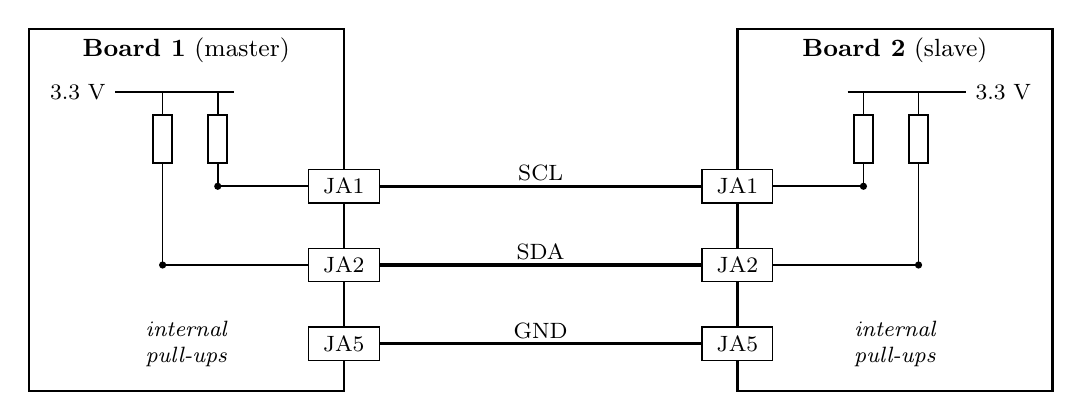
\begin{tikzpicture}
% boards
\node[draw, line width=0.8pt, minimum width=4.0cm, minimum height=4.6cm] (b1) at (0,0) {};
\node[draw, line width=0.8pt, minimum width=4.0cm, minimum height=4.6cm] (b2) at (9,0) {};
\node[anchor=north, align=center, font=\small] at (b1.north) {\textbf{Board 1} (master)};
\node[anchor=north, align=center, font=\small] at (b2.north) {\textbf{Board 2} (slave)};
% pins on the Pmod JA edge
\foreach \y/\t/\k in {0.3/JA1/scl, -0.7/JA2/sda, -1.7/JA5/gnd} {
  \node[draw, fill=white, font=\footnotesize, minimum width=0.9cm] (L\k) at (2.0,\y) {\t};
  \node[draw, fill=white, font=\footnotesize, minimum width=0.9cm] (R\k) at (7.0,\y) {\t};
}
\draw[line width=1.1pt] (Lscl) -- node[lab,above]{SCL} (Rscl);
\draw[line width=1.1pt] (Lsda) -- node[lab,above]{SDA} (Rsda);
\draw[line width=1.1pt] (Lgnd) -- node[lab,above]{GND} (Rgnd);
% internal pull-ups, board 1
\draw[dg] (-0.9,1.5) -- (0.6,1.5); \node[font=\footnotesize, anchor=east] at (-0.9,1.5) {3.3 V};
\pullup{0.4}{1.5}{0.3} \draw[dg] (0.4,0.3) -- (Lscl.west);
\pullup{-0.3}{1.5}{-0.7} \draw[dg] (-0.3,-0.7) -- (Lsda.west);
% internal pull-ups, board 2
\draw[dg] (8.4,1.5) -- (9.9,1.5); \node[font=\footnotesize, anchor=west] at (9.9,1.5) {3.3 V};
\pullup{8.6}{1.5}{0.3} \draw[dg] (8.6,0.3) -- (Rscl.east);
\pullup{9.3}{1.5}{-0.7} \draw[dg] (9.3,-0.7) -- (Rsda.east);
\node[font=\footnotesize\itshape, align=center] at (0,-1.7) {internal\\pull-ups};
\node[font=\footnotesize\itshape, align=center] at (9,-1.7) {internal\\pull-ups};
\end{tikzpicture}\end{document}
